%!TEX program = xelatex
%!TEX options=--shell-escape
\documentclass[12pt]{article}

%
\usepackage[scheme=plain]{ctex}
%
\usepackage{fontspec}
%
\usepackage[margin = 1in]{geometry}

%
\usepackage[dvipsnames]{xcolor}
\usepackage[many]{tcolorbox}

%
\usepackage{amsmath}
\usepackage{amssymb}
\usepackage{amsthm}
%
\usepackage{tensor}
%
\usepackage{slashed}
\usepackage{physics}
\usepackage{simpler-wick}

%
\usepackage[version=4]{mhchem}

%
\usepackage{mathtools}

%
\usepackage{bm}
\newcommand{\dbar}{\dif\hspace*{-0.18em}\bar{}\hspace*{0.2em}}
\DeclareMathAlphabet\mathbfcal{OMS}{cmsy}{b}{n}
%\usepackage{bbold}
\newcommand*{\dif}{\mathop{}\!\mathrm{d}}
\newcommand*{\euler}{\mathrm{e}}
\newcommand*{\imagi}{\mathrm{i}}

\renewcommand{\vec}[1]{\boldsymbol{\mathbf{#1}}}

\usepackage{caption}
\usepackage{multirow}
\usepackage{enumitem}

%
\usepackage{mathrsfs}
\usepackage{dsfont}

%
\usepackage{hyperref}
\hypersetup{
    colorlinks=true,
    linkcolor=violet,
    filecolor=blue,      
    urlcolor=blue,
    citecolor=cyan,
}

%
\usepackage{graphicx}
\usepackage{subfig}
%
\graphicspath{{image/}}


%
\usepackage{indentfirst}
%
\setlength{\parindent}{2em}
\linespread{1.25}

% 
% \setmainfont{Times New Roman}

\title{Note}
\author{Feng-Yang Hsieh}
\date{}

\begin{document}
\maketitle

\section{SPANet2}% (fold)
\label{sec:spanet2}
	Version 2 of SPANet. call it SPANet2. 
	\subsection{Defining event topology}% (fold)
	\label{sub:defining_event_topology}
		Defining the event topology in \verb+.ymal+ file. The structure of the \verb+.yaml+ file follows this format:
		\begin{verbatim}
		INPUTS:
		    SEQUENTIAL:
		\end{verbatim}
	% subsection defining_event_topology (end)
	\subsection{Creating training dataset}% (fold)
	\label{sub:creating_training_dataset}
		\verb+.hdf5+
	% subsection creating_training_dataset (end)
	\subsection{Training options}% (fold)
	\label{sub:training_options}
		
	% subsection training_options (end)
	\subsection{Training}% (fold)
	\label{sub:training}
		Training:
		\begin{verbatim}
			python -m spanet.train -of <OPTIONS_FILE> --log_dir <LOG_DIR>  --name <NAME> 
		\end{verbatim}
		\verb+<OPTIONS_FILE>+: JSON file with options. \verb+<LOG_DIR>+: output directory. \verb+<NAME>+: subdirectory name

		Evaluation:
		\begin{verbatim}
			python -m spanet.test <log_directory> -tf <TEST_FILE>
		\end{verbatim}
		\verb+<log_directory>+: directory containing the checkpoint and options file.  \verb+<TEST_FILE>+ will replace the test file in the option file.

		Prediction:
		\begin{verbatim}
			python predict.py <log_directory> <output name> -tf <TEST_FILE> --gpu ???
		\end{verbatim}
	
	% subsection training (end)
% section spanet2 (end)
\section{Test SPANet2}% (fold)
\label{sec:test_spanet2}
	\subsection{SM SPANet}% (fold)
	\label{sub:sm_spanet}
		Generate the correct format $\kappa_\lambda = 1$ training data for SPANet2 training.
		\begin{itemize}
			\item Training sample:
			\begin{itemize}
				\item Total sample size: 76,131
				\item 1h sample size: 14,527
				\item 2h sample size: 60,122
				\item 5\% used on validation
			\end{itemize}
			\item Testing sample:
			\begin{itemize}
				\item Total sample size: 8,460
				\item 1h sample size: 1,577
				\item 2h sample size: 6,744
			\end{itemize}
		\end{itemize}
		The training results are presented in Table \ref{tab:SPANet2_diHiggs_4btag_DL1r_pt40_k1}.
		\begin{table}[htpb]
			\centering
			\caption{SPA-NET2 training results on the SM di-Higgs samples.}
			\label{tab:SPANet2_diHiggs_4btag_DL1r_pt40_k1}
			\begin{tabular}{c|c|cc}
				$N_\text{Jet}$ & Event Fraction & Event Efficiency & Higgs Efficiency \\
				\hline
				$=4$	  &   0.280             &    0.907              &    0.907             \\
				$=5$	  &   0.287             &    0.806              &    0.847             \\
				$\ge 6$	  &   0.229             &    0.679              &    0.753             \\
				Total	  &   0.797             &    0.805              &    0.841             \\
			\end{tabular}
		\end{table}

	% subsection sm_spanet (end)
	\subsection{\texorpdfstring{$\kappa 5$}{kappa 5} SPANet}% (fold)
	\label{sub:kappa_5_spanet}
		Generate the $\kappa_\lambda = 5$ training data for SPANet2 training.
		\begin{itemize}
			\item Training sample:
			\begin{itemize}
				\item Total sample size: 78,388
				\item 1h sample size: 16,013
				\item 2h sample size: 59,180
				\item 5\% used on validation
			\end{itemize}
			\item Testing sample: 
			\begin{itemize}
				\item Total sample size: 8,710
				\item 1h sample size: 1,846
				\item 2h sample size: 6,486
			\end{itemize}
		\end{itemize}
		The training results are presented in Table \ref{tab:SPANet2_diHiggs_4btag_DL1r_pt40_k5}.
		\begin{table}[htpb]
			\centering
			\caption{SPA-NET2 training results on the di-Higgs $\kappa_\lambda =5$ samples.}
			\label{tab:SPANet2_diHiggs_4btag_DL1r_pt40_k5}
			\begin{tabular}{c|c|cc}
				$N_\text{Jet}$ & Event Fraction & Event Efficiency & Higgs Efficiency \\
				\hline
				$=4$	  &   0.315             &    0.689              &    0.689             \\
				$=5$	  &   0.255             &    0.617              &    0.639             \\
				$\ge 6$	  &   0.174             &    0.499              &    0.544             \\
				Total	  &   0.745             &    0.620              &    0.638             \\
			\end{tabular}
		\end{table}

	% subsection kappa_5_spanet (end)
	\subsection{Resonant SPANet}% (fold)
	\label{sub:resonant_spanet}
		Generate the correct format resonant training data for SPANet2 training.
		\begin{itemize}
			\item Training sample:
			\begin{itemize}
				\item Total sample size: 51,145
				\item 1h sample size: 9,320
				\item 2h sample size: 40,991
				\item 5\% used on validation
			\end{itemize}
			\item Testing sample:
			\begin{itemize}
				\item Total sample size: 5,683
				\item 1h sample size: 1,011
				\item 2h sample size: 4,582
			\end{itemize}
		\end{itemize}
		The training results are presented in Table \ref{tab:SPANet2_diHiggs_4btag_DL1r_pt40_res}.
		\begin{table}[htpb]
			\centering
			\caption{SPA-NET2 training results on the resonant di-Higgs samples.}
			\label{tab:SPANet2_diHiggs_4btag_DL1r_pt40_res}
			\begin{tabular}{c|c|cc}
				$N_\text{Jet}$ & Event Fraction & Event Efficiency & Higgs Efficiency \\
				\hline
				$=4$	  &   0.316             &    0.930              &    0.930             \\
				$=5$	  &   0.282             &    0.808              &    0.839             \\
				$\ge 6$	  &   0.208             &    0.660              &    0.727             \\
				Total	  &   0.806             &    0.818              &    0.846             \\
			\end{tabular}
		\end{table}

	% subsection resonant_spanet (end)

	\subsection{Mixing \texorpdfstring{$\kappa_\lambda$}{kappa} SPANet}% (fold)
	\label{sub:mixing_kappa_spanet}
		Generate the correct format mixing $\kappa_\lambda$ training data for SPANet2 training.
		\begin{itemize}
			\item Training sample:
			\begin{itemize}
				\item Total sample size: 51,145
				\item 1h sample size: 9,320
				\item 2h sample size: 40,991
				\item 5\% used on validation
			\end{itemize}
			\item Testing sample:
			\begin{itemize}
				\item Total sample size: 5,683
				\item 1h sample size: 1,011
				\item 2h sample size: 4,582
			\end{itemize}
		\end{itemize}
		The training results are presented in Table \ref{tab:SPANet2_diHiggs_4btag_DL1r_pt40_mix}.
		\begin{table}[htpb]
			\centering
			\caption{SPA-NET2 training results on the resonant di-Higgs samples.}
			\label{tab:SPANet2_diHiggs_4btag_DL1r_pt40_mix}
			\begin{tabular}{c|c|cc}
				$N_\text{Jet}$ & Event Fraction & Event Efficiency & Higgs Efficiency \\
				\hline
				$=4$	  &   0.316             &    0.930              &    0.930             \\
				$=5$	  &   0.282             &    0.808              &    0.839             \\
				$\ge 6$	  &   0.208             &    0.660              &    0.727             \\
				Total	  &   0.806             &    0.818              &    0.846             \\
			\end{tabular}
		\end{table}

		
	% subsection mixing_kappa_spanet (end)
	\subsection{Summary}% (fold)
	\label{sub:summary}
		In most cases, the performance of SPANet2 is worse than the old one. Some default options are different between the two versions. But even if the options are set as identical, the training results also cannot be better.

		The training results of old and new versions SPANet have been summarized in Table \ref{tab:training_results_of_SPANET_12}.
		\begin{table}[htpb]
			\centering
			\caption{SPA-NET2 training results on the resonant di-Higgs samples.}
			\label{tab:training_results_of_SPANET_12}
			\begin{tabular}{c|cc}
						 & \multicolumn{2}{c}{Event efficiency} \\
						 & SPANet           & SPANet2           \\ \hline
			SM           & 0.868            & 0.805             \\
			kappa 5      & 0.725            & 0.620             \\
			Resonant     & 0.903            & 0.818             \\
			Mixing $\kappa_\lambda$& 0.833            & 0.830            
			\end{tabular}
		\end{table}

	% subsection summary (end)

% section test_spanet2 (end)
\section{Combine jet assignment and event classification}% (fold)
\label{sec:combine_jet_assignment_and_event_classification}
	This section trains the SPANet2 on the jet assignment and event classification task at the same time. This is the new feature of SPANet2.
	\subsection{\texorpdfstring{$\kappa_\lambda=5$}{kappa 5} sample}% (fold)
	\label{sub:kappa_5_sample}
		For the jet assignment part, use the same sample as in Sec. \ref{sub:kappa_5_spanet}. 
		\begin{itemize}
			\item Training sample:
			\begin{itemize}
				\item Total sample size: 168,125
				\item Signal sample size: 78,388
				\item Background sample size: 89,737
				\item 5\% used on validation
			\end{itemize}
			\item Testing sample:
			\begin{itemize}
				\item Total sample size: 18,681
				\item Signal sample size: 8,710
				\item Background sample size: 9,971
			\end{itemize}
		\end{itemize}

		The training results are presented in Table \ref{tab:SPANet2_diHiggs_4b_pt40_k5_class}.
		\begin{table}[htpb]
			\centering
			\caption{SPA-NET2 training results on the $\kappa_\lambda =5$ samples.}
			\label{tab:SPANet2_diHiggs_4b_pt40_k5_class}
			\begin{tabular}{c|c|cc}
				$N_\text{Jet}$ & Event Fraction & Event Efficiency & Higgs Efficiency \\
				\hline
				$=4$	  &   0.316             &    0.930              &    0.930             \\
				$=5$	  &   0.282             &    0.808              &    0.839             \\
				$\ge 6$	  &   0.208             &    0.660              &    0.727             \\
				Total	  &   0.806             &    0.818              &    0.846             \\
			\end{tabular}
		\end{table}	

	% subsection kappa_5_sample (end)
	\subsection{Mixing \texorpdfstring{$\kappa_\lambda$}{kappa}}% (fold)
	\label{sub:mixing_kappa}
		\subsubsection{Training samples}% (fold)
		\label{subs:training_samples}
			For signal, set $\kappa_\lambda = [-5, -3, -1, 1, 2, 3, 5, 7, 9, 12]$ and generate 9,000 samples on each $\kappa_\lambda$ point for training. The training samples are required to pass the ``Four tag cut'', i.e., there are at least four b-tagged jets with $p_\text{T} > \text{40 GeV}$ and $\abs{\eta} < 2.5$. 

			Note that the $\kappa_\lambda$ value is an input feature. For the background sample, the input $\kappa_\lambda$ value is randomly chosen from the above values.

			For the jet assignment part,
			\begin{itemize}
				\item Training sample:
				\begin{itemize}
					\item Total sample size: 90,000
					\item 1h sample size: 18,020
					\item 2h sample size: 69,267
					\item 5\% used on validation
				\end{itemize}
				\item Testing sample:
				\begin{itemize}
					\item Total sample size: 9,000
					\item 1h sample size: 1,802
					\item 2h sample size: 6,899				
				\end{itemize}
			\end{itemize}

			For event classification,
			\begin{itemize}
				\item Training sample:
				\begin{itemize}
					\item Total sample size: 179,737
					\item Signal sample size: 90,000
					\item Background sample size: 89,737
					\item 5\% used on validation
				\end{itemize}
				\item Testing sample:
				\begin{itemize}
					\item Total sample size: 18,971
					\item Signal sample size: 9,000
					\item Background sample size: 9,971
				\end{itemize}
			\end{itemize}
		% subsubsection training_samples (end)
		\subsubsection{Hyperparameters setting}% (fold)
		\label{subs:hyperparameters_setting}
			Some options are different between SPANet and SPANet2. List the different options below
			\begin{itemize}
				\item \verb+hidden_dim+: $128 \to 64$ 
				\item \verb+learning_rate+: $0.0007 \to 0.0015$ 
				\item \verb+num_attention_heads+: $8 \to 4$ 
			\end{itemize}

			The total loss function consists of assignment loss and classification loss. The same weights are assigned to these losses.
			\begin{itemize}
				\item \verb+assignment_loss_scale+: 1.0
				\item \verb+classification_loss_scale+: 1.0
			\end{itemize}
		% subsubsection hyperparameters_setting (end)		
		\subsubsection{Training results}% (fold)
		\label{subs:training_results}
			The jet assignment training results are presented in Table \ref{tab:SPANet2_diHiggs_4b_pt40_mix_class}.
			\begin{table}[htpb]
				\centering
				\caption{SPANet2 training results on the mixing $\kappa_\lambda$ samples.}
				\label{tab:SPANet2_diHiggs_4b_pt40_mix_class}
				\begin{tabular}{c|c|cc}
					$N_\text{Jet}$ & Event Fraction & Event Efficiency & Higgs Efficiency \\
					\hline
					$=4$	  &   0.139             &    0.866              &    0.866             \\
					$=5$	  &   0.130             &    0.806              &    0.834             \\
					$\ge 6$	  &   0.095             &    0.704              &    0.766             \\
					Total	  &   0.364             &    0.802              &    0.829             \\
				\end{tabular}
			\end{table}	

			The classification training results are presented in Table \ref{tab:SPANET_cls_results}.
			\begin{table}[htpb]
				\centering
				\caption{The SPANet2 classification training results with mixing $\kappa_\lambda$ sample.}
				\label{tab:SPANET_cls_results}
				\begin{tabular}{c|cc}
				Training sample        & ACC     & AUC   \\ \hline
				Mixing $\kappa_\lambda $ & $0.828$ & $0.911$
				\end{tabular}      
			\end{table}

		% subsubsection training_results (end)		
	% subsection mixing_kappa (end)	
% section combine_jet_assignment_and_event_classification (end)		
\section{\texorpdfstring{$\kappa_\lambda$}{kappa} constraints on SPANet2}% (fold)
\label{sec:kappa_constraints_on_spanet2}

	\subsection{SPANet2 classification}% (fold)
	\label{sub:spanet2_classification}
		Use the SPANet2 to do the signal background classification task. 

		When an event is put in SPANet2, SPANet2 will return a signal score $p_\text{signal}$ which represents the confidence of this event is a signal event. The requirement of $p_\text{signal} > p_\text{th}$ is imposed for event selection, where $p_\text{th} = 0.90$. In where do not choose the value which can maximize the $S / \sqrt{B}$. Because the value is too close to $1$, then very few events can pass this selection. Thus we can not do further analysis.  

		Set the $\kappa_\lambda$ limits by the profile likelihood method and CLs method. Table \ref{tab:kappa_constraint_SPANet} results from $\kappa_\lambda$ constraints.
		\begin{table}[htpb]
			\centering
			\caption{The $\kappa_\lambda$ constraints of SPANet2.}
			\label{tab:kappa_constraint_SPANet}
			\begin{tabular}{c|cc|cc}
								  & \multicolumn{4}{c}{Expected Constraint}                          \\
								  & \multicolumn{2}{c}{Profile likelihood} & \multicolumn{2}{c}{CLs} \\ \hline
			Selection method        & Lower              & Upper             & Lower      & Upper      \\ \hline
			SPANet2      & $-3.48$            & $9.18$             & $-3.41$      & $9.09$      \\
			\end{tabular}
		\end{table}

	% subsection spanet2_classification (end)
		
% section kappa_constraints_on_spanet2 (end)	
\section{Comparision with previous results}% (fold)
\label{sec:comparision_with_previous_results}
	This section summary the results among the ``$\text{min-}\Delta R$ DNN'', ``$\kappa 5$ SPANet DNN'', ``mixing $\kappa$ SPANet2''.
	\subsection{Pairing performance}% (fold)
	\label{sub:pairing_performance}
		Figure \ref{fig:pairing_performance_kappa} is the pairing efficiency of different pairing methods. Where the mixing $\kappa$ SPANet2 has the best performance.
		\begin{figure}[htpb]
			\centering
			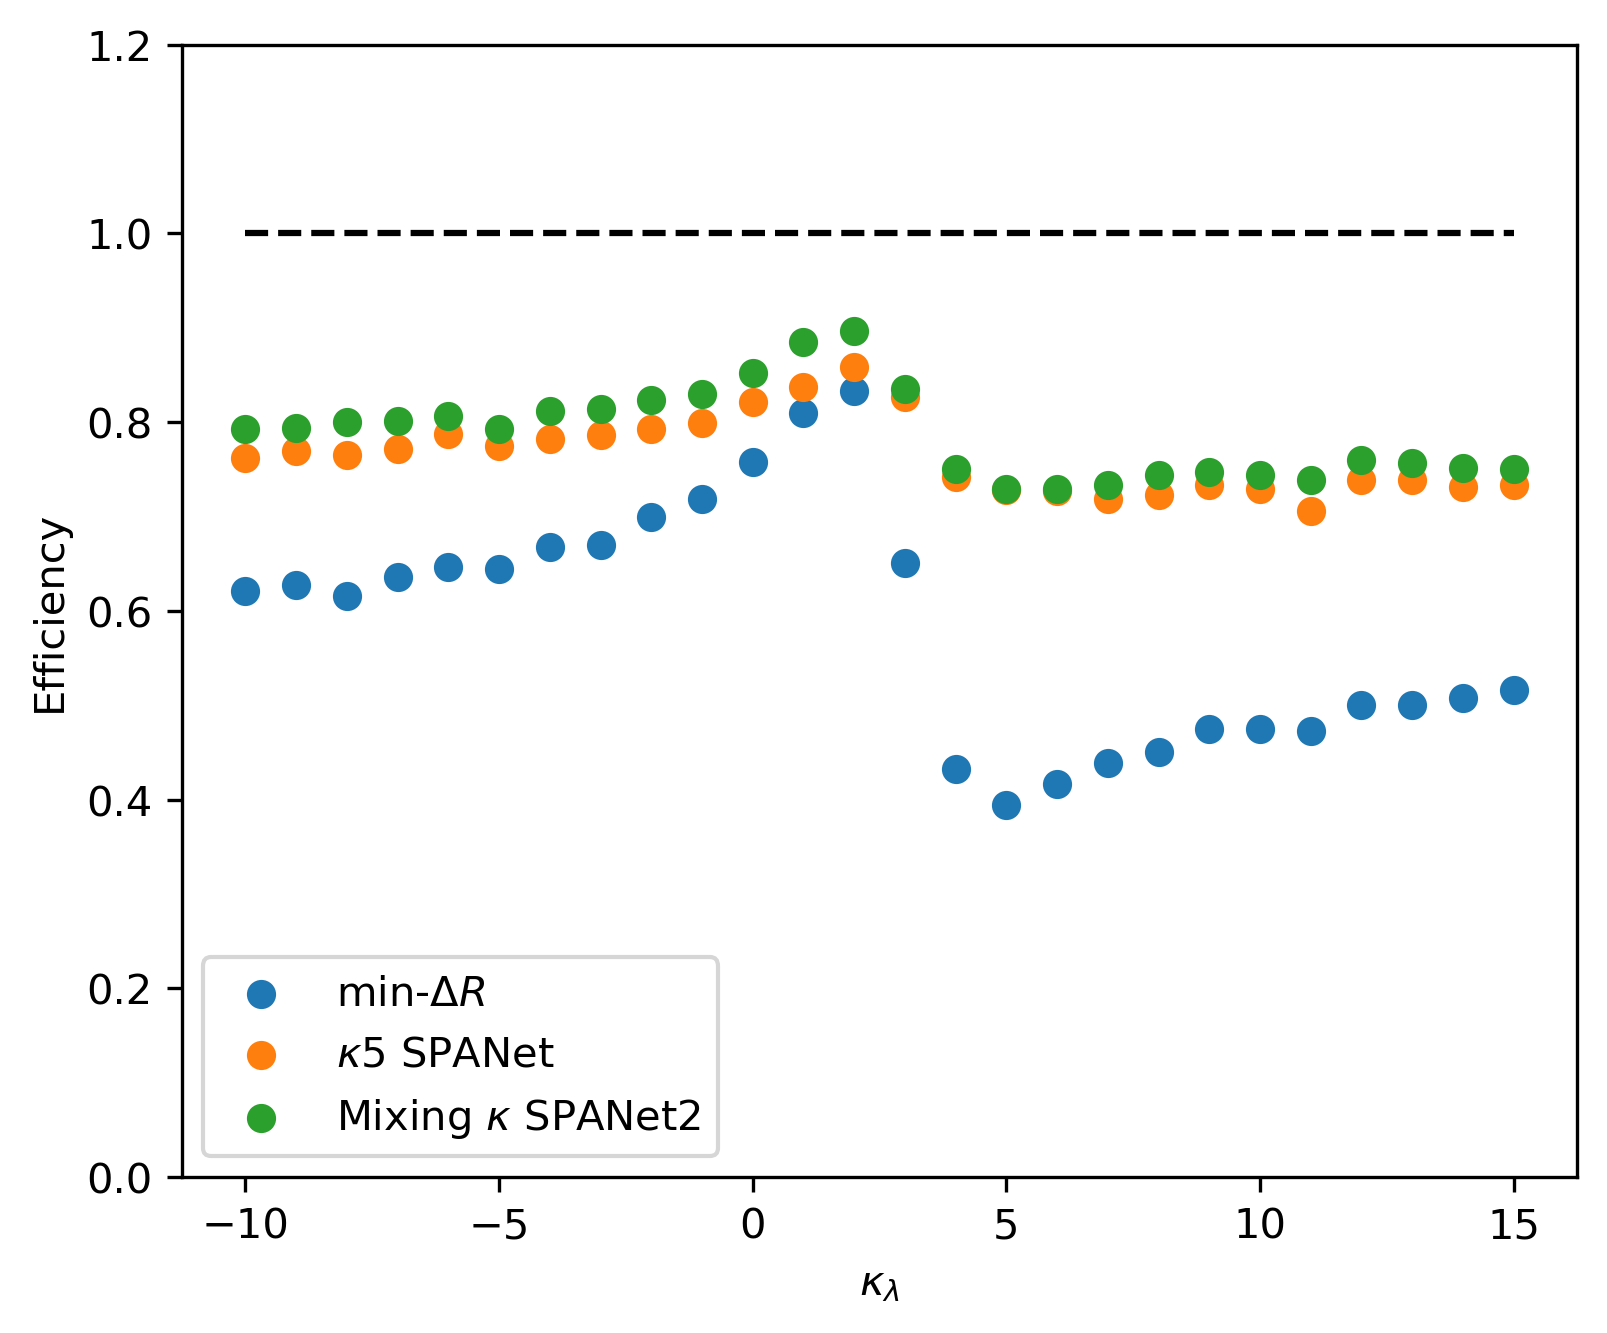
\includegraphics[width=0.65\textwidth]{pairing_efficiency_kappa-SPANet2.png}
			\caption{The pairing performance for different $\kappa_\lambda$ samples.}
			\label{fig:pairing_performance_kappa}
		\end{figure}

	% subsection pairing_performance (end)
	\subsection{Classification performance}% (fold)
	\label{sub:classification_performance}
		The classification training results are presented in Table \ref{tab:SPANET_cls_results}.
		\begin{table}[htpb]
			\centering
			\caption{The classification performance of different selection methods.}
			\label{tab:classification_results_summary}
			\begin{tabular}{c|cc}
			Selection method          & ACC   & AUC   \\ \hline
			$\text{min-}\Delta R$ DNN & 0.783 & 0.864 \\
			$\kappa 5$ SPANet DNN     & 0.792 & 0.875 \\
			mixing $\kappa$ SPANet2   & 0.828 & 0.911
			\end{tabular}			
		\end{table}

	% subsection classification_performance (end)
	\subsection{\texorpdfstring{$\kappa_\lambda$}{kappa} constraints}% (fold)
	\label{sub:kappa_constraints}
		Table \ref{tab:kappa_constraint_summary} is the $\kappa_\lambda$ constraints of the different selection methods.
		\begin{table}[htpb]
			\centering
			\caption{The $\kappa_\lambda$ constraints of different selection methods.}
			\label{tab:kappa_constraint_summary}
			\begin{tabular}{cc|cc|cc}
									&                  & \multicolumn{4}{c}{Expected Constraints}                         \\
									&                  & \multicolumn{2}{c}{Profile likelihood} & \multicolumn{2}{c}{CLs} \\ \hline
			Pairing method          & Selection method & Lower              & Upper             & Lower       & Upper     \\ \hline
			$\text{min-}\Delta R$   & DNN              & $-3.81$            & $11.16$           & $-3.73$     & $11.15$   \\
			$\kappa 5$ SPANet       & DNN              & $-4.08$            & $11.65$           & $-4.02$     & $11.68$   \\
			Mixing $\kappa$ SPANet2 & SPANet2          & $-3.48$            & $9.18$            & $-3.41$     & $9.09$   
			\end{tabular}		
		\end{table}


	% subsection kappa_constraints (end)
	\subsection{Mass distribution plot}% (fold)
	\label{sub:mass_distribution_plot}
		Figure \ref{fig:Higgs_mass_signal} and \ref{fig:Higgs_mass_background} show the Higgs mass distribution for signal and background events with different pairing methods. The selection does not apply. The mass planes for the signal process all look similar for all pairing methods. For background, the results of $\text{min-}\Delta R$ are very different from others.
		\begin{figure}[htpb]
			\centering
			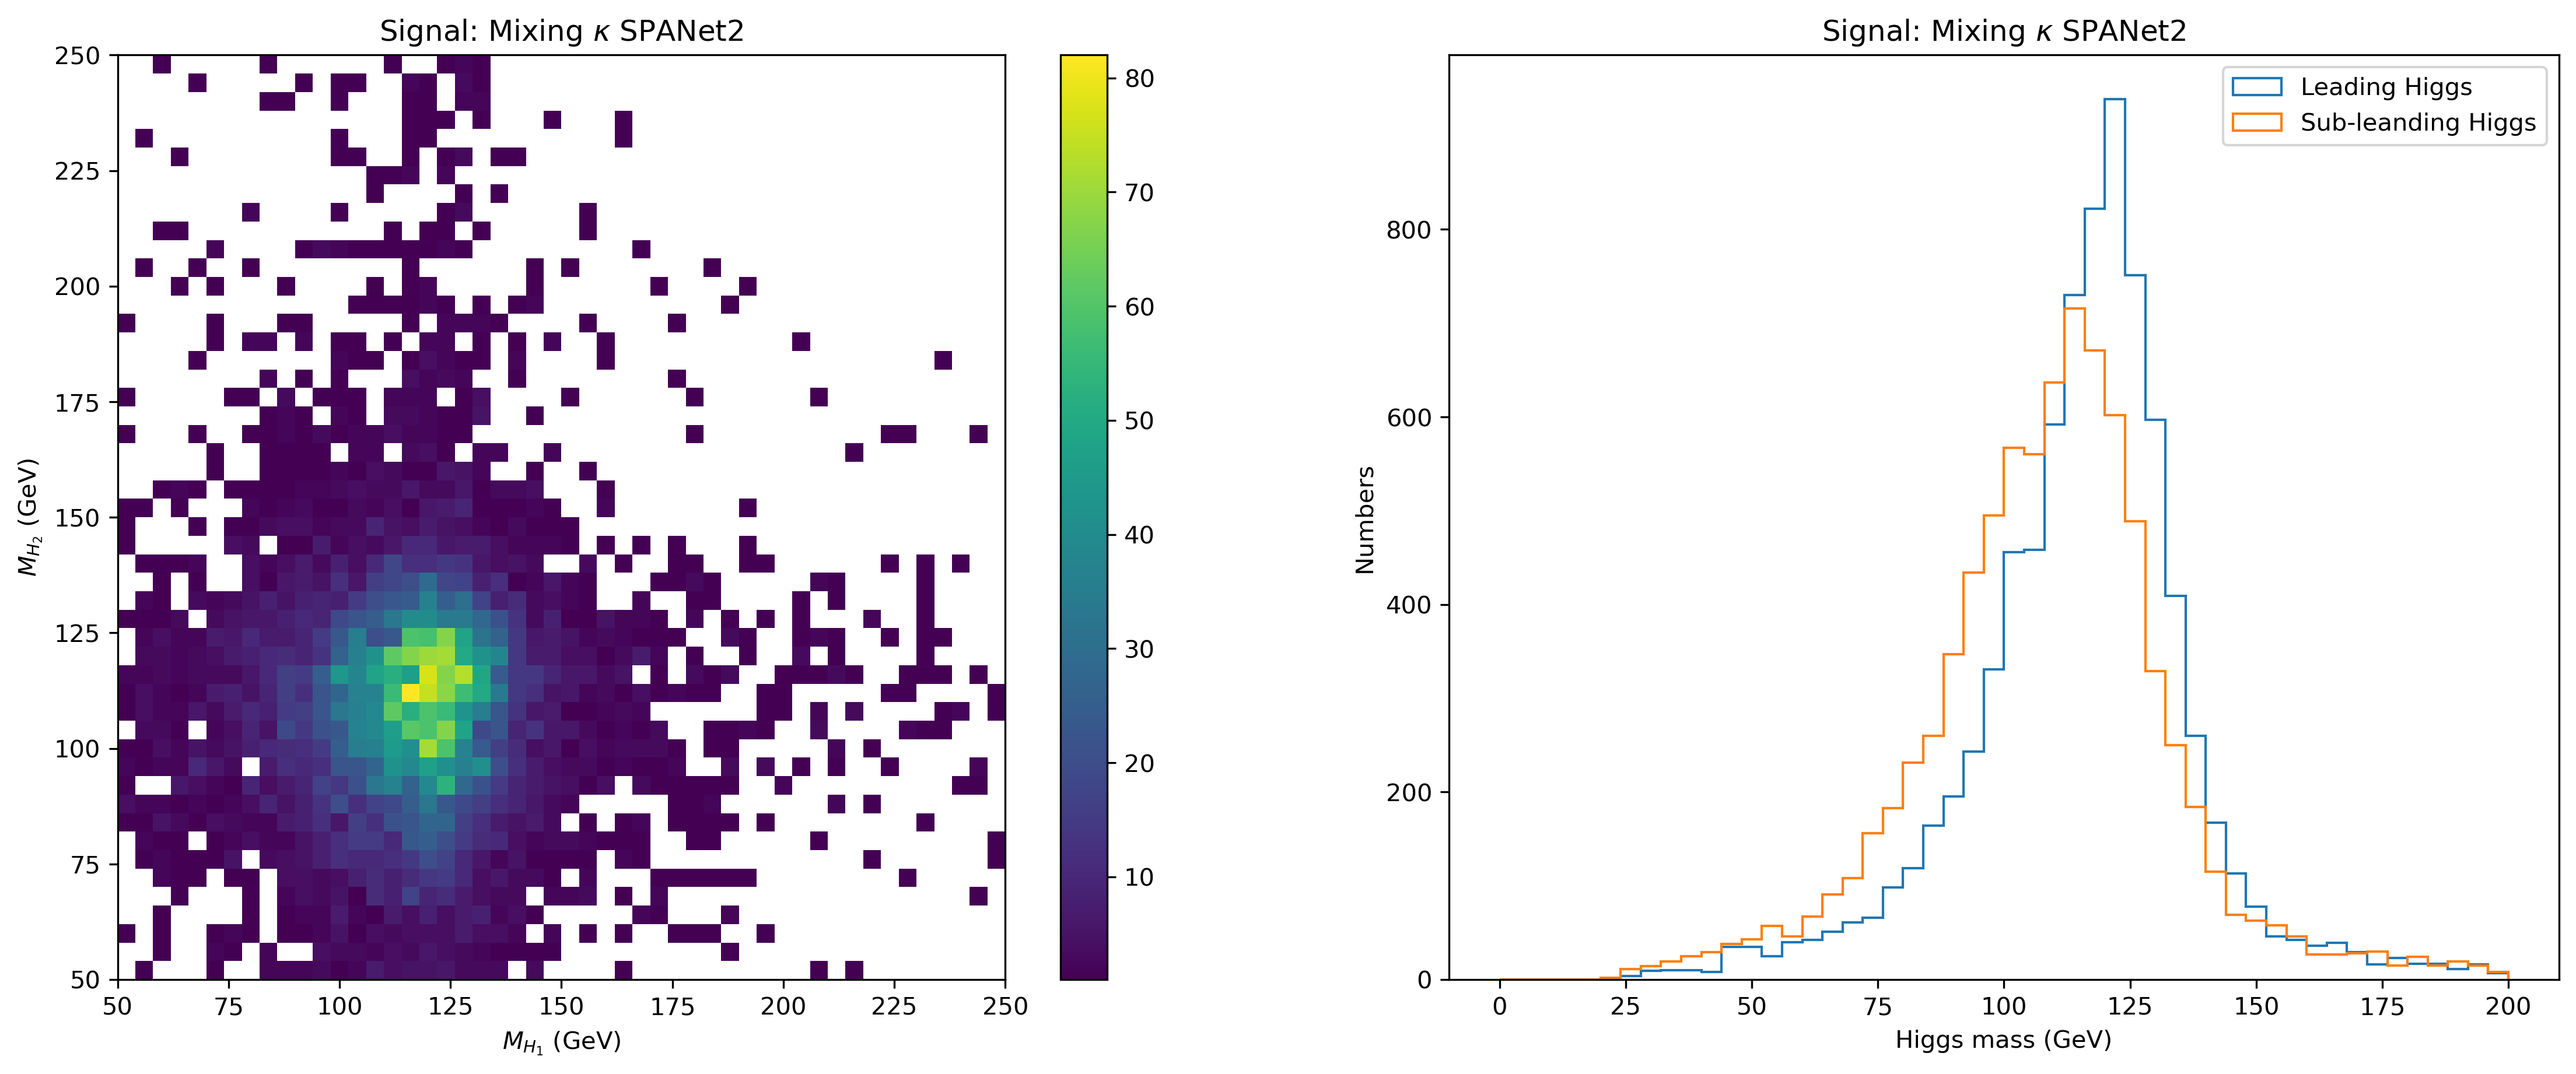
\includegraphics[width=0.97\textwidth]{Higgs_mass_mix-SPANET2_s.png}
			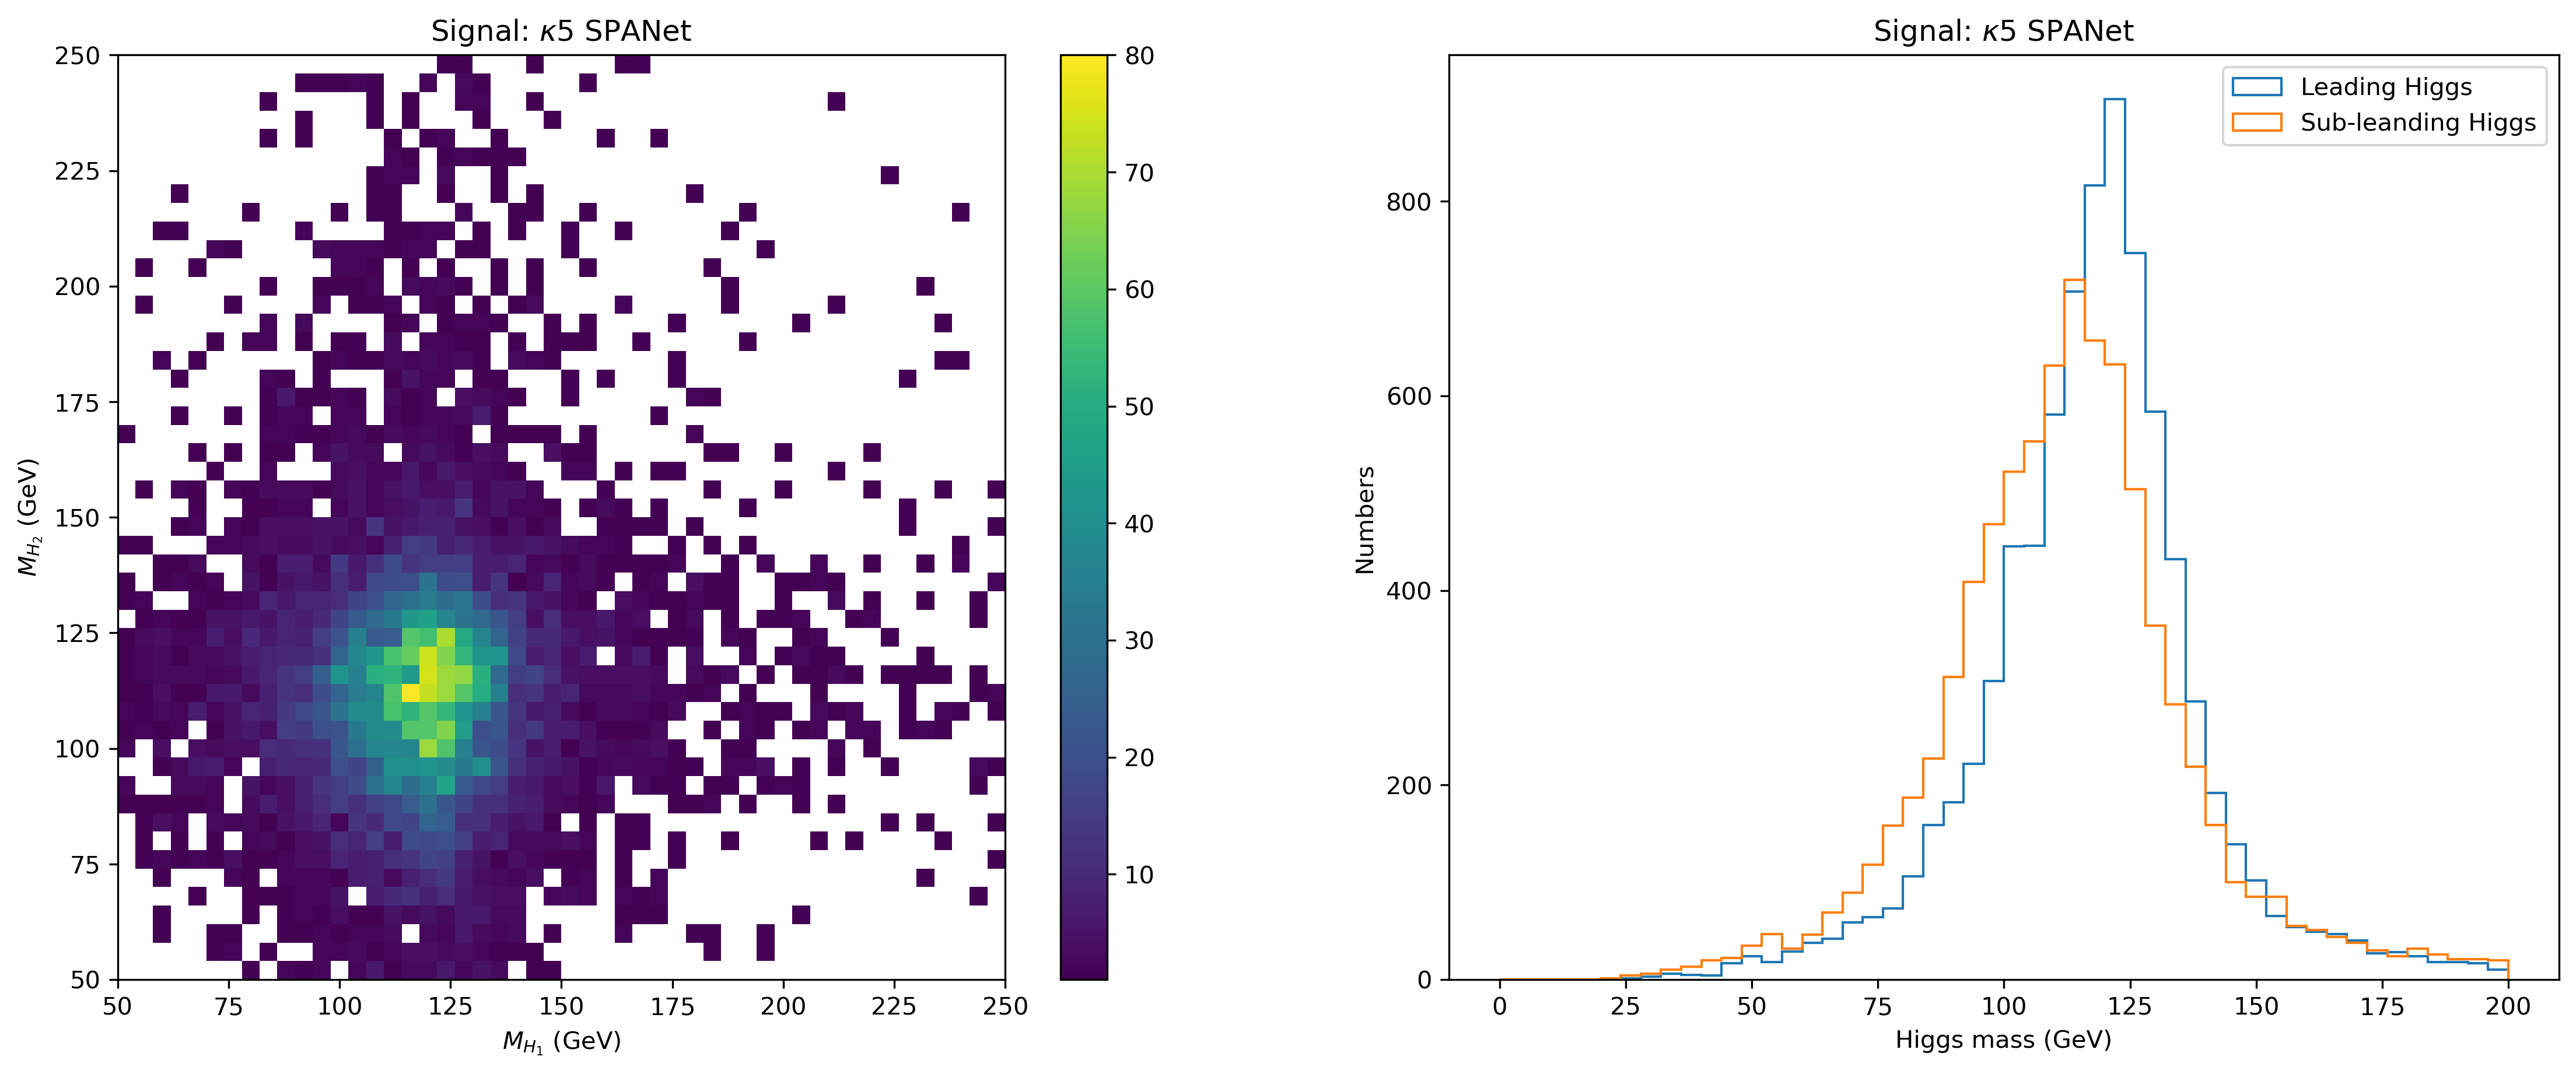
\includegraphics[width=0.97\textwidth]{Higgs_mass_k5-SPANET_s.png}
			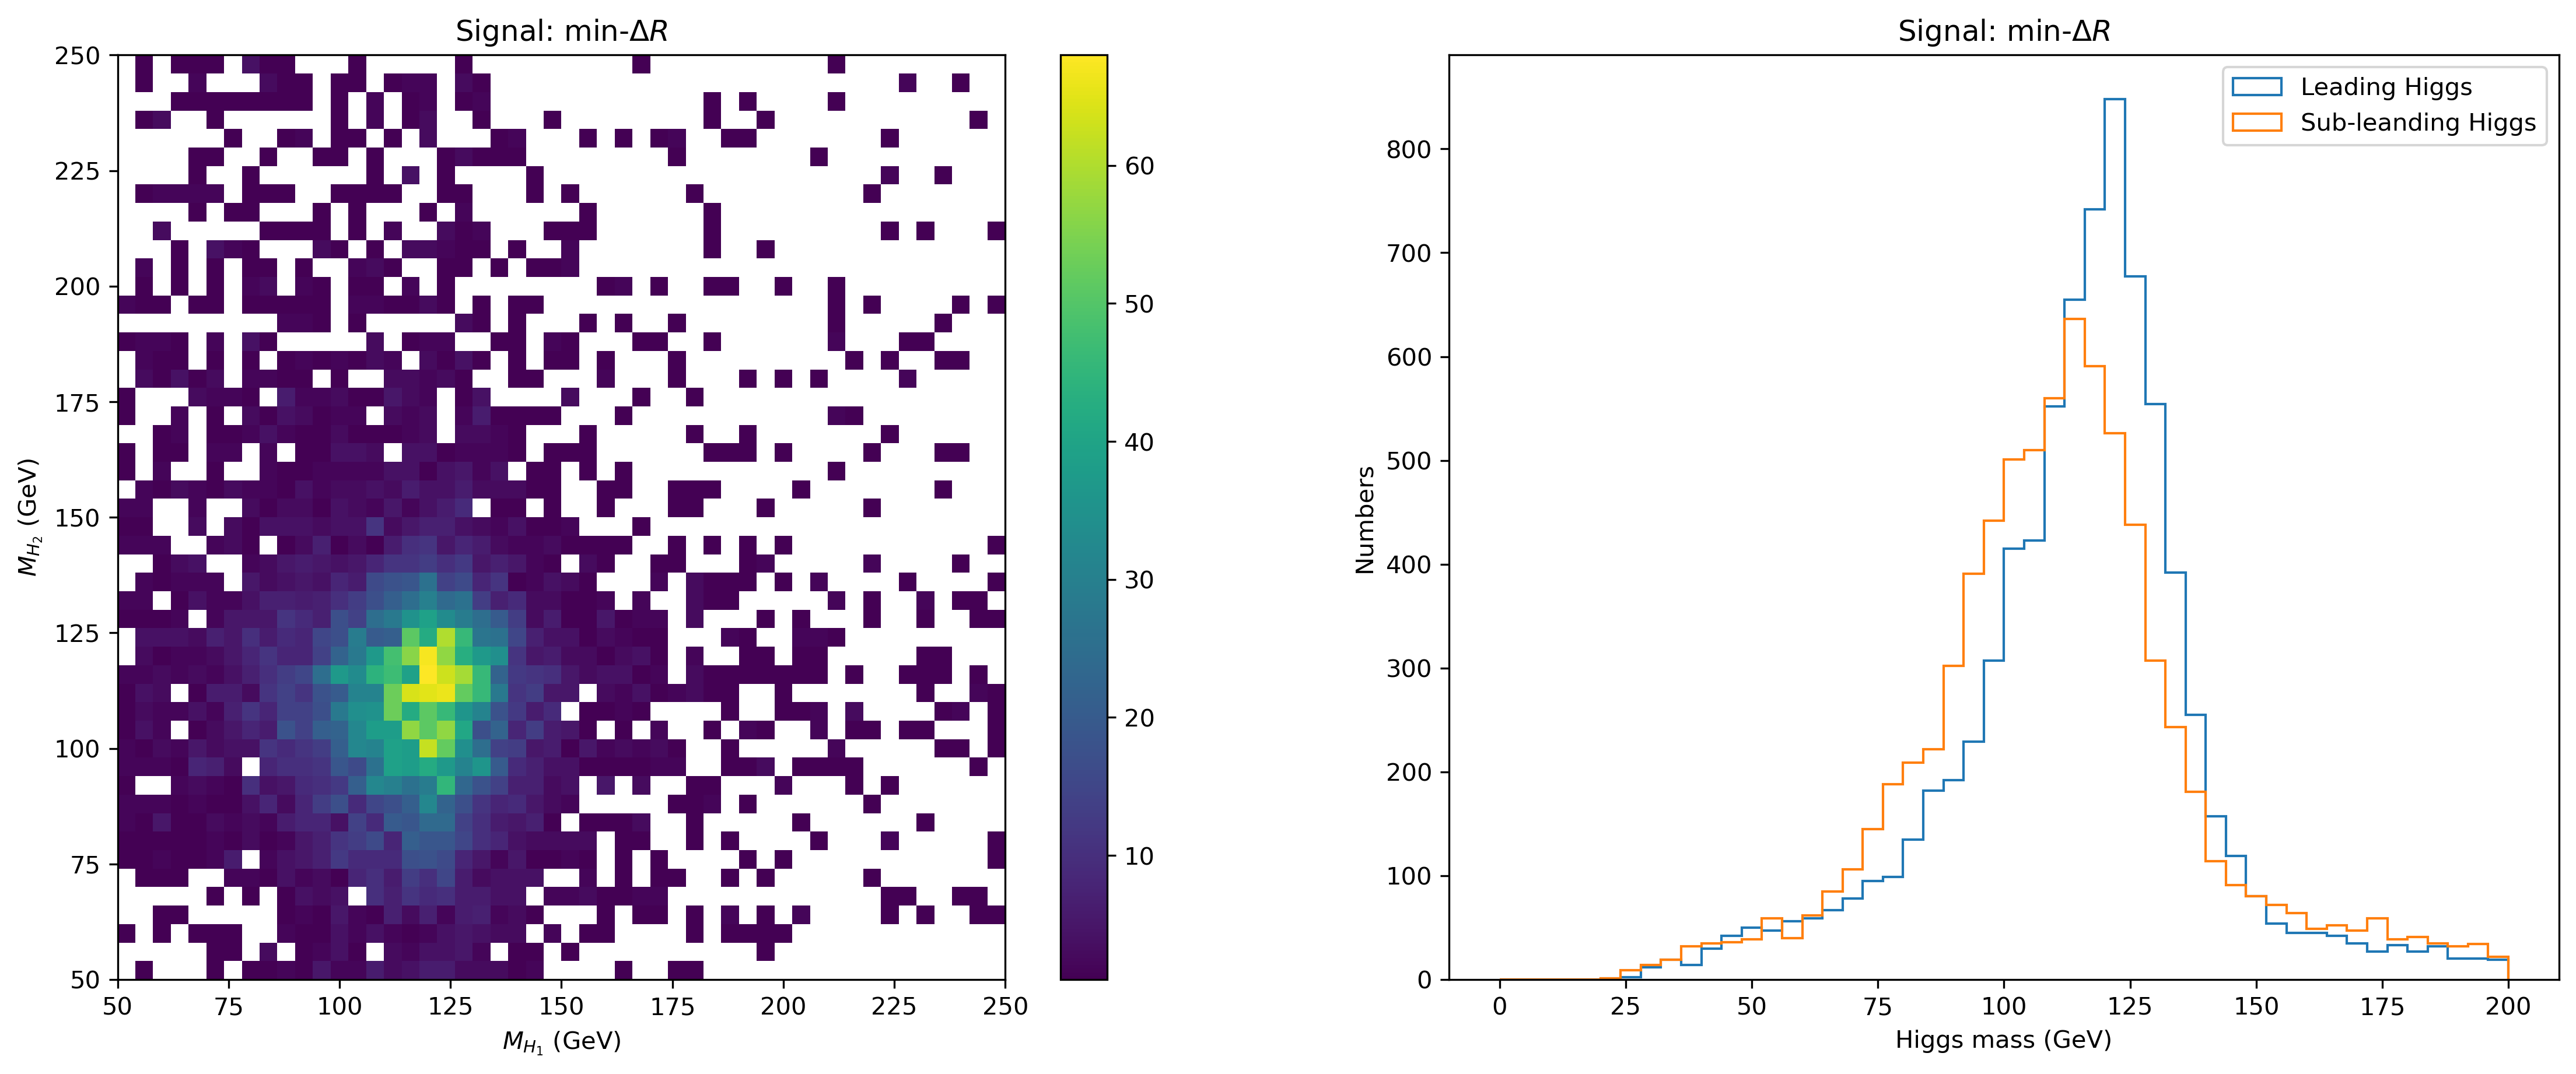
\includegraphics[width=0.97\textwidth]{Higgs_mass_mindR_s.png}
			\caption{The mass plane and distribution of Higgs candidate for signal events with different pairing methods. The top one is mixing $\kappa$ SPANet2 pairing, the middle one is $\kappa 5$ SPANet pairing, bottom one is $\text{min-}\Delta R$ pairing.}
			\label{fig:Higgs_mass_signal}
		\end{figure}

		\begin{figure}[htpb]
			\centering
			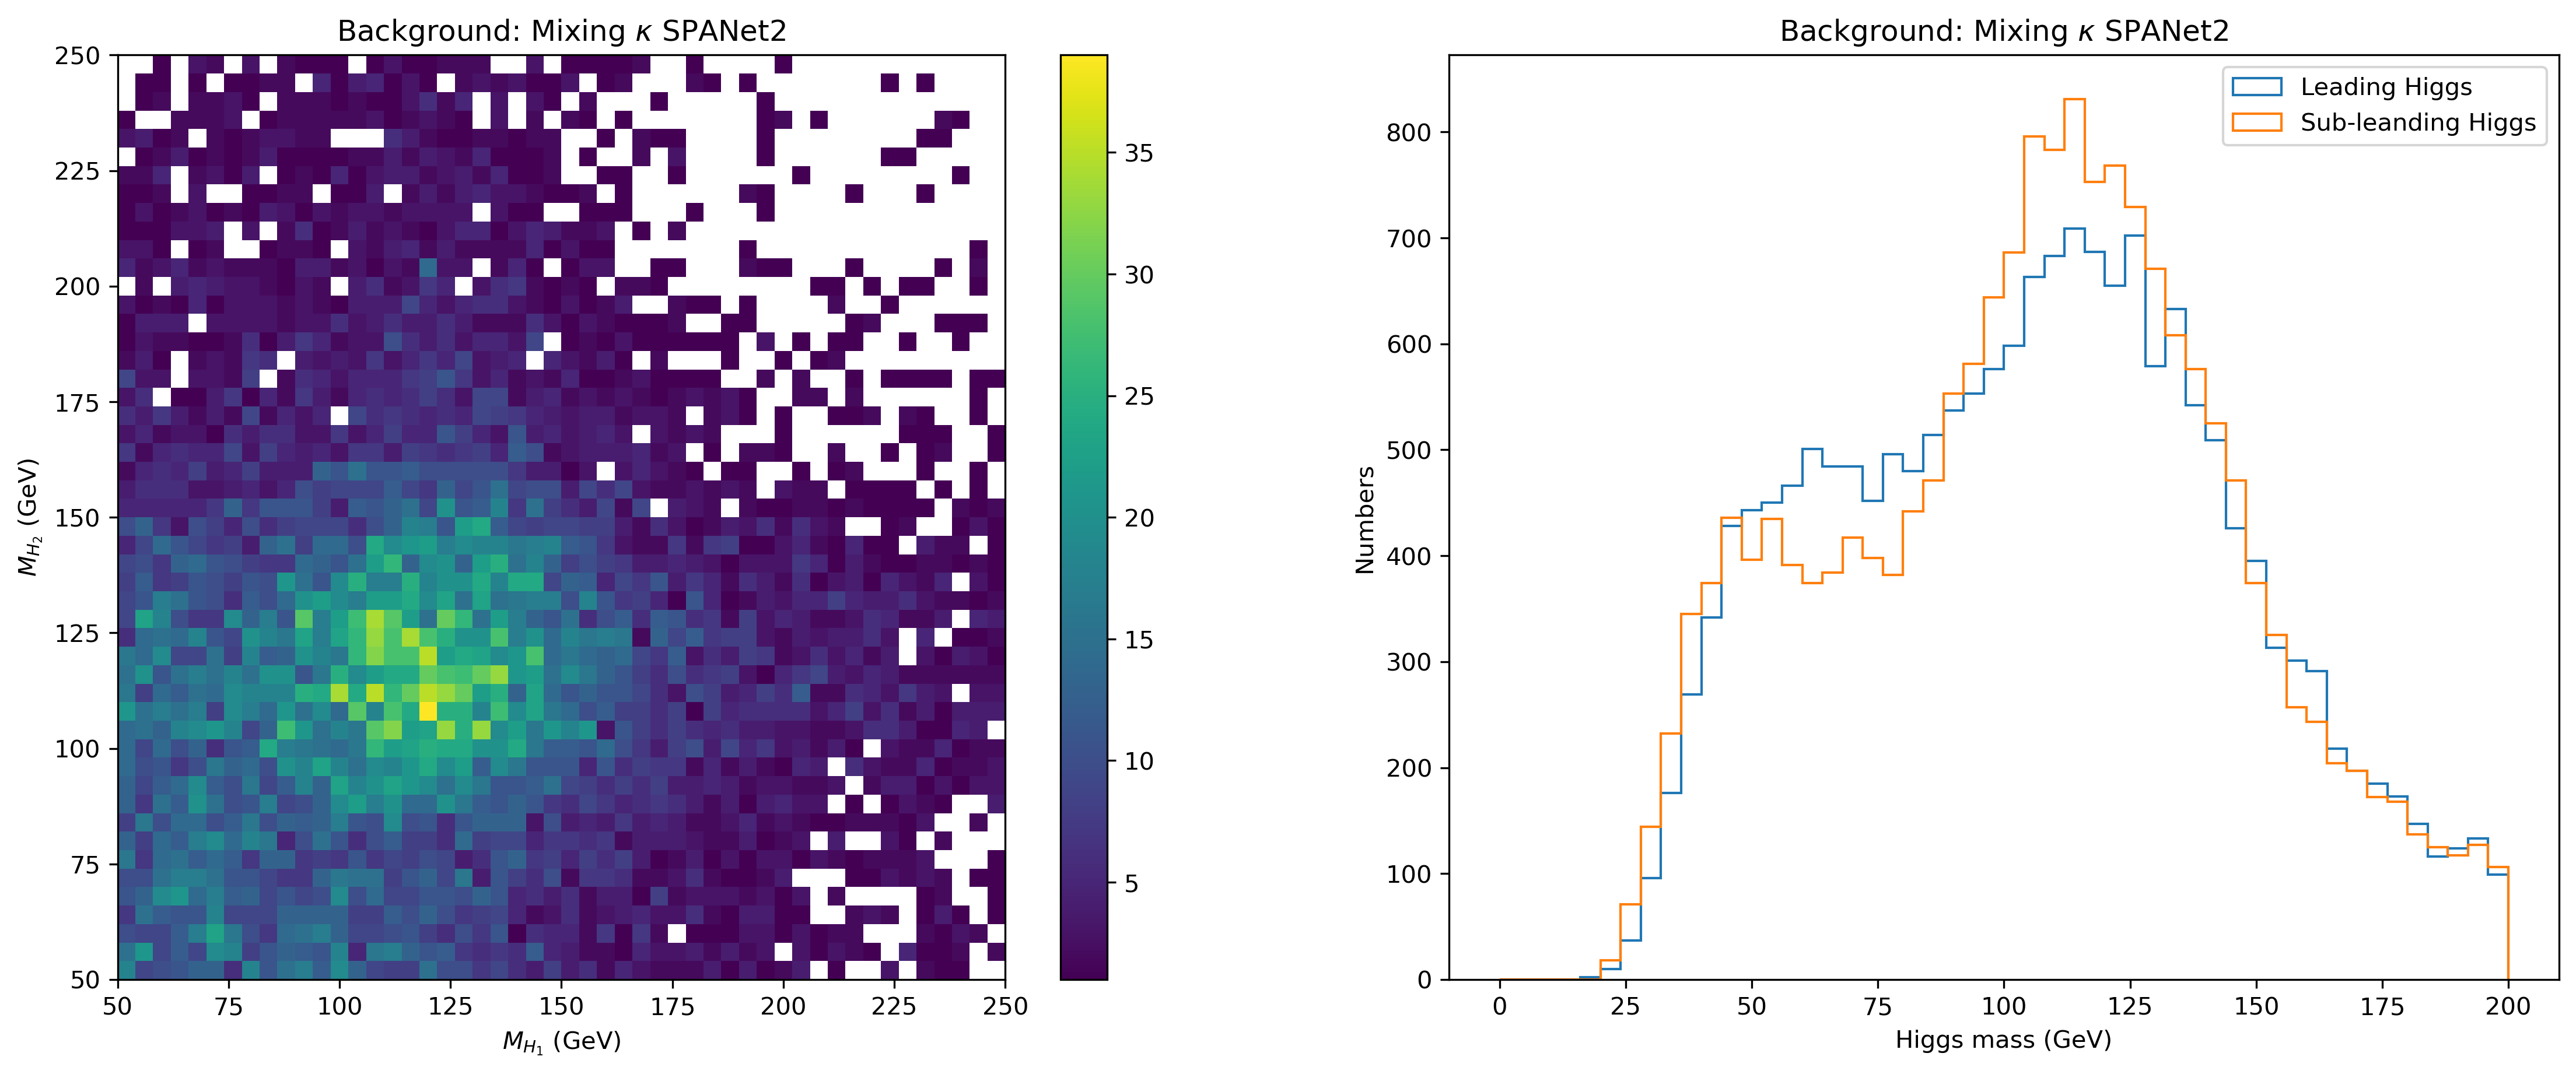
\includegraphics[width=0.97\textwidth]{Higgs_mass_mix-SPANET2_b.png}
			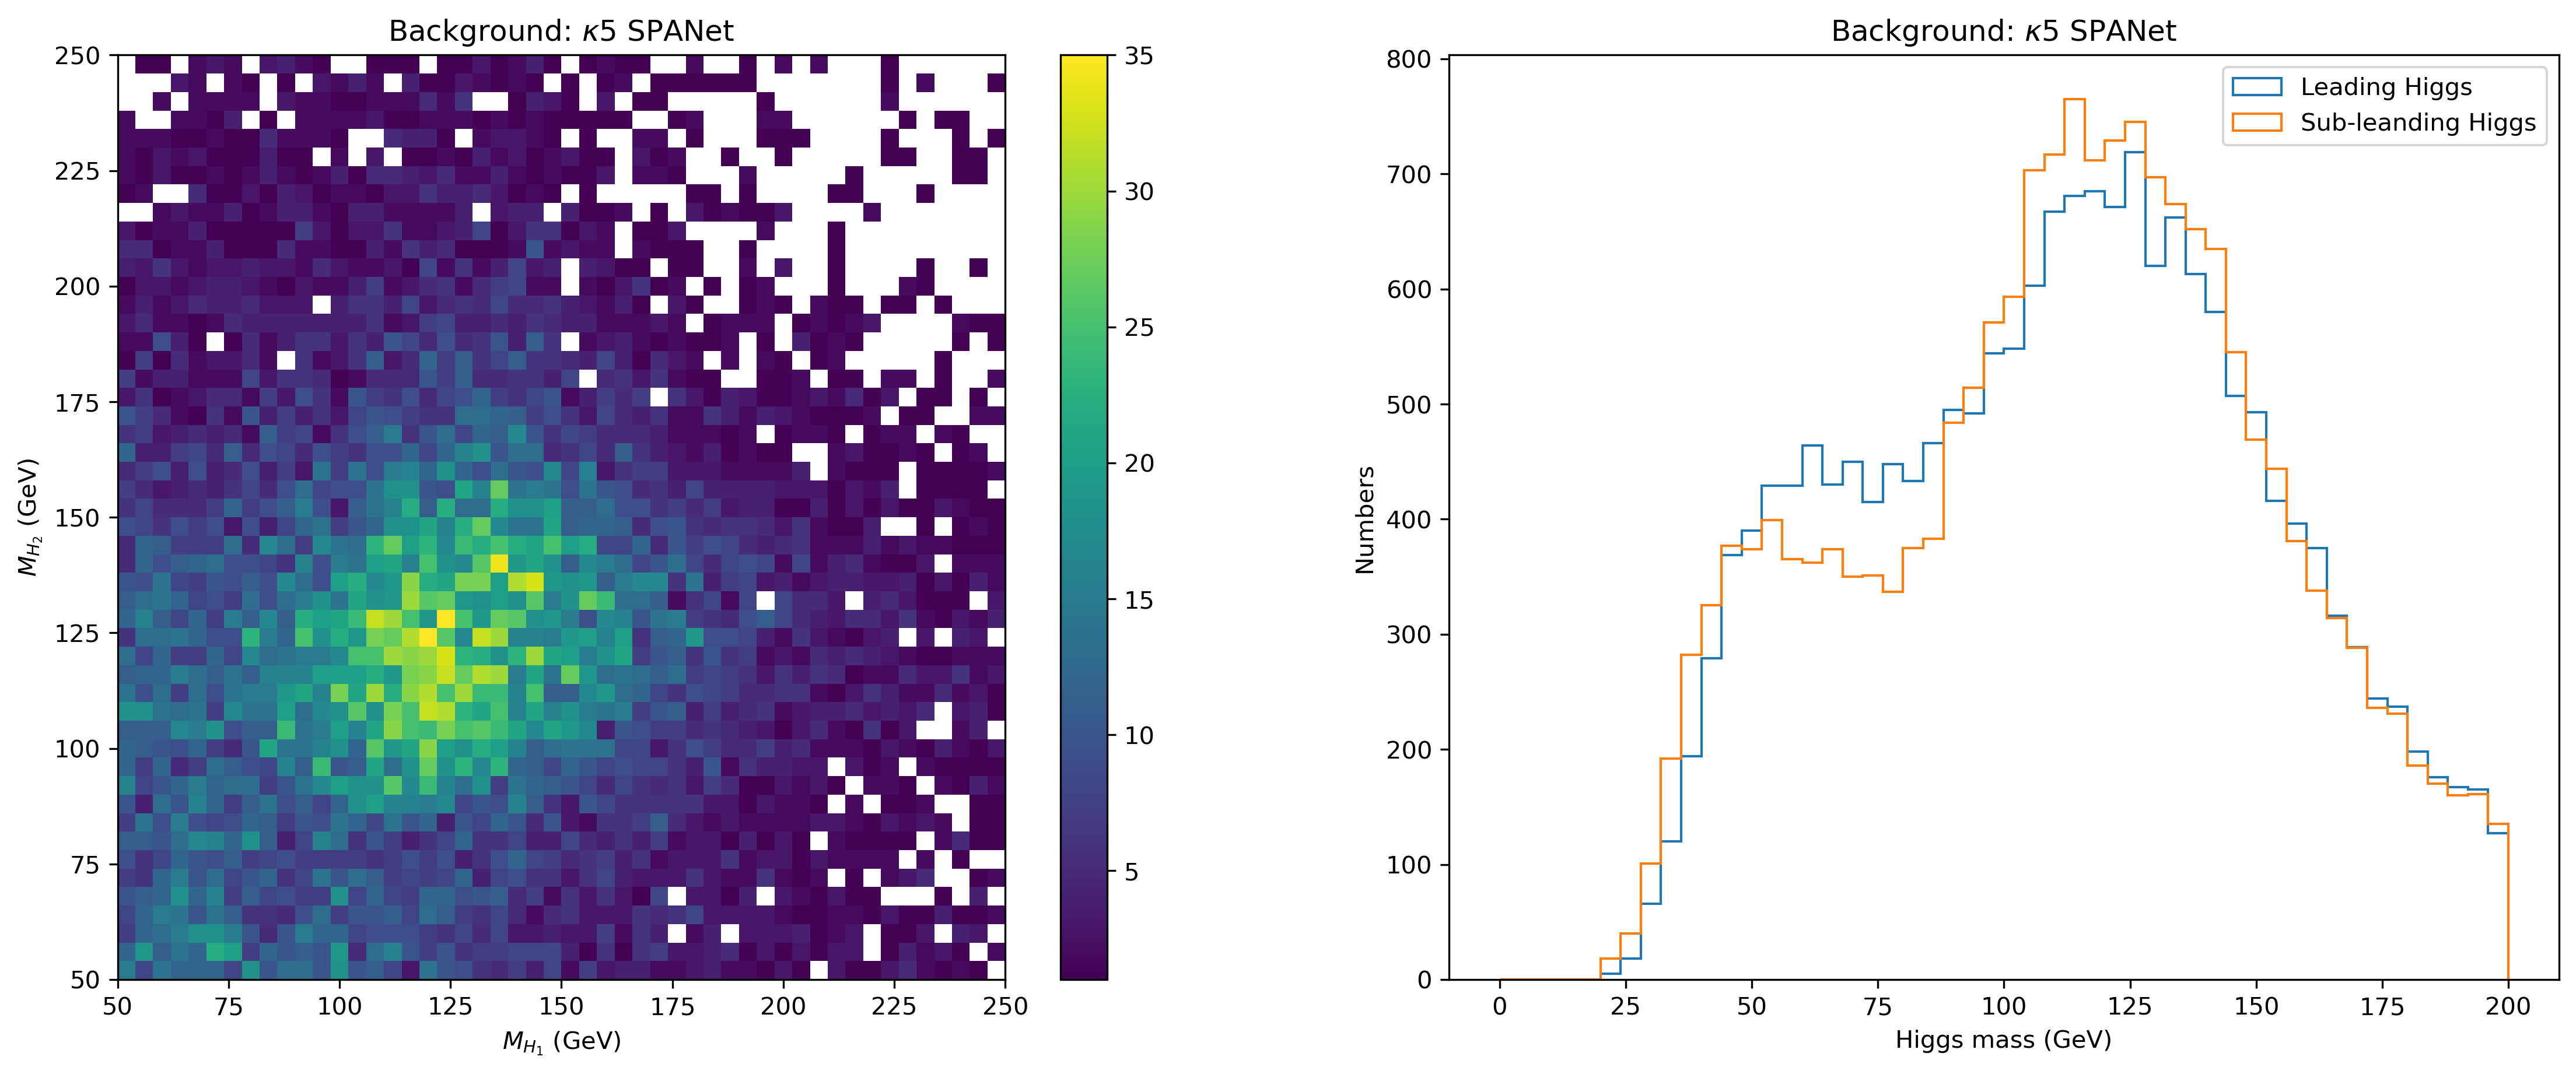
\includegraphics[width=0.97\textwidth]{Higgs_mass_k5-SPANET_b.png}
			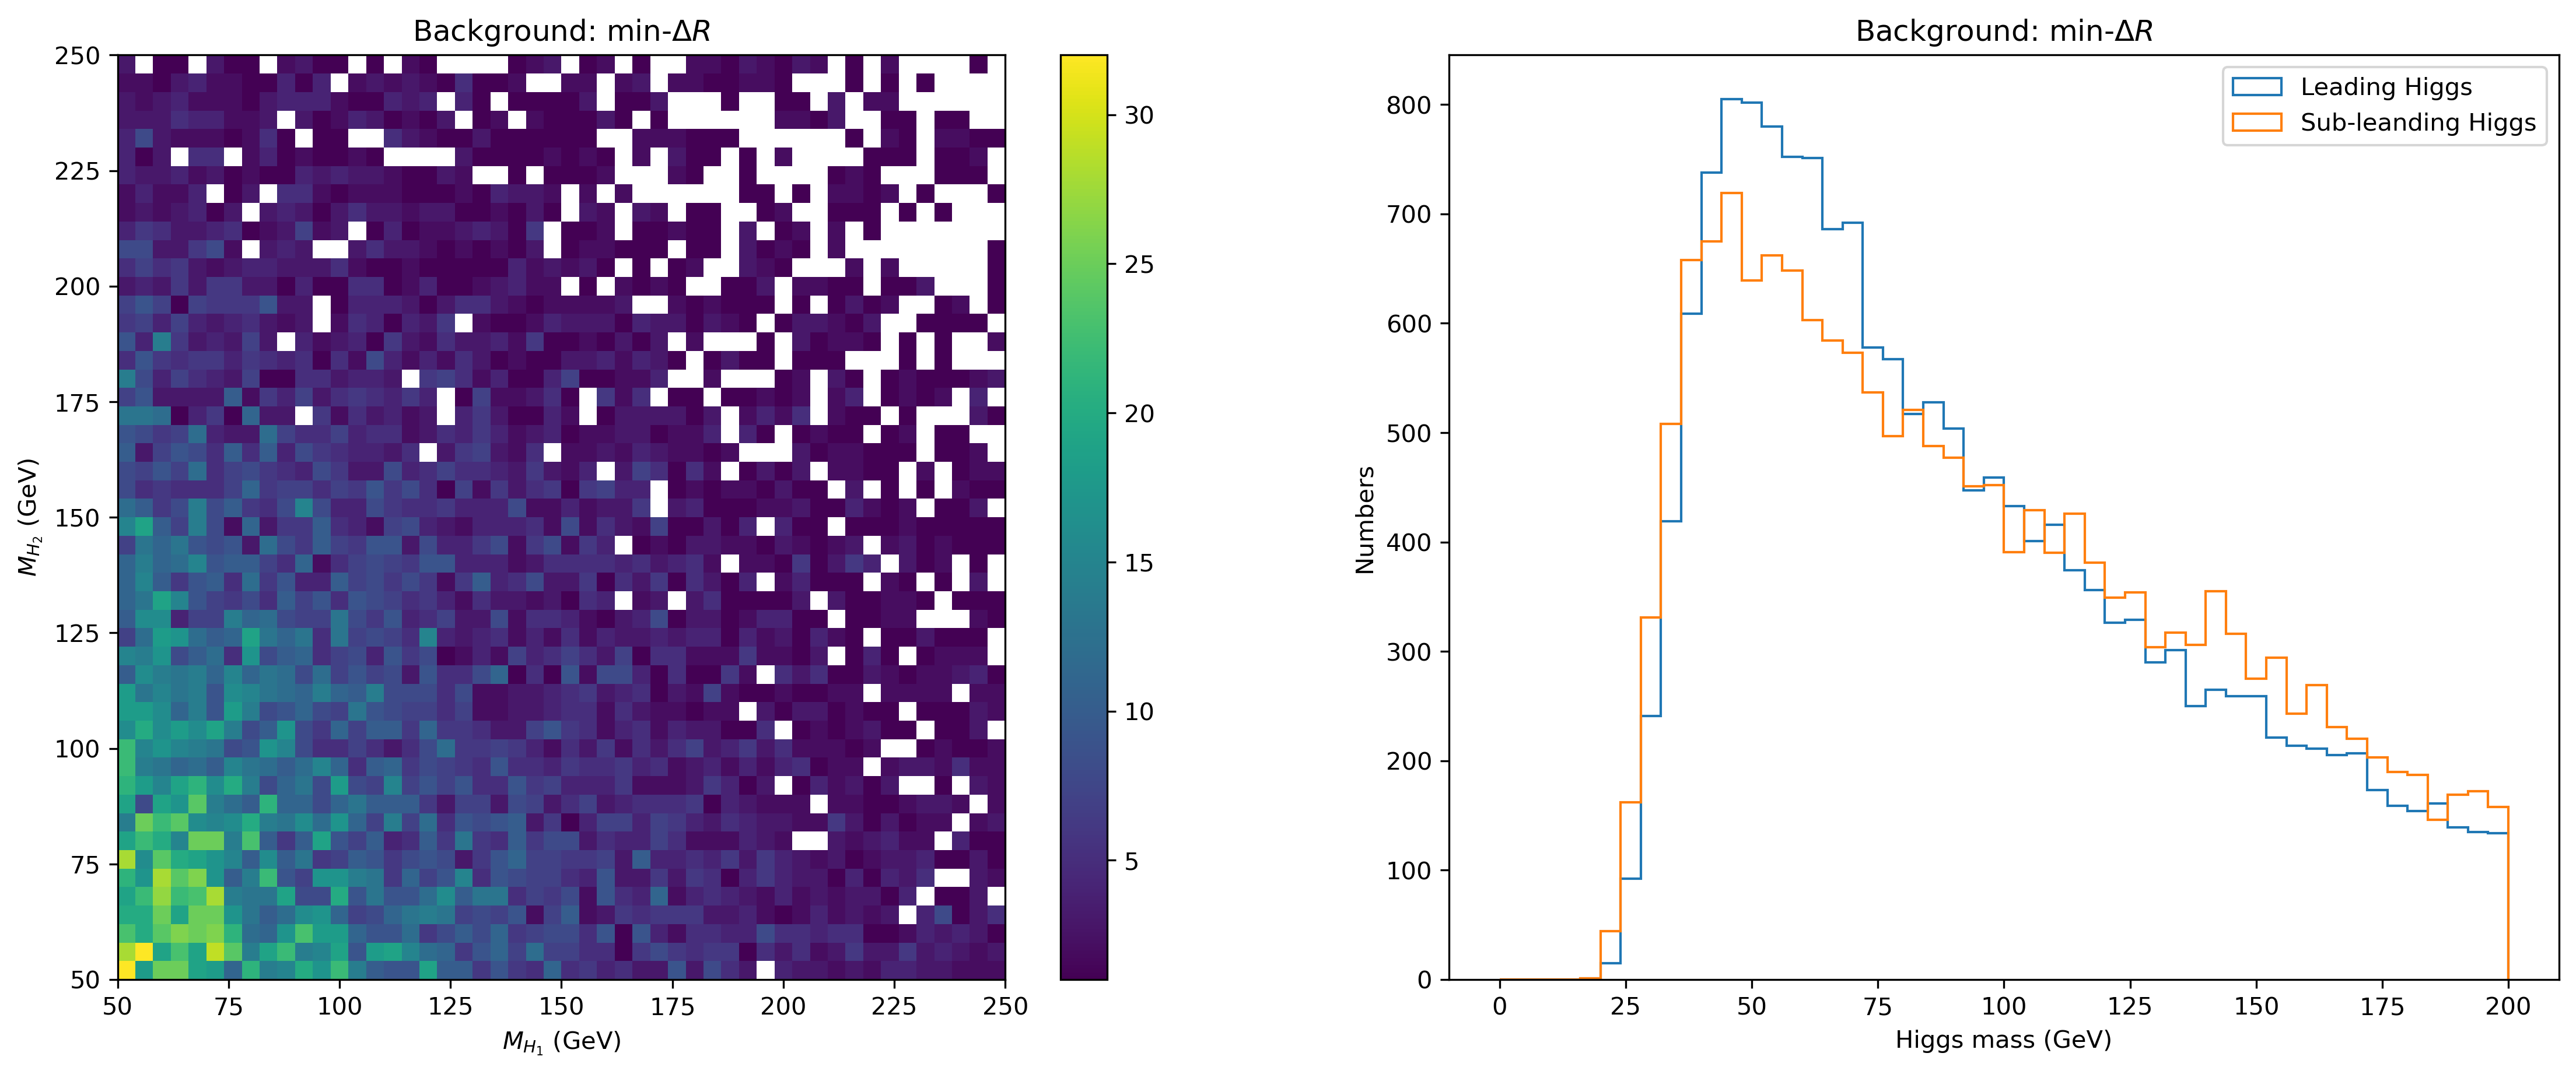
\includegraphics[width=0.97\textwidth]{Higgs_mass_mindR_b.png}
			\caption{The mass plane and distribution of Higgs candidate for background events with different pairing methods. The top one is mixing $\kappa$ SPANet2 pairing, the middle one is $\kappa 5$ SPANet pairing, bottom one is $\text{min-}\Delta R$ pairing.}
			\label{fig:Higgs_mass_background}
		\end{figure}


		Figure \ref{fig:mhh_distributions} are the $m_{HH}$ distributions after the selection.
		\begin{figure}[htpb]
			\centering
			\subfloat[$\text{min-}\Delta R$ DNN]{
				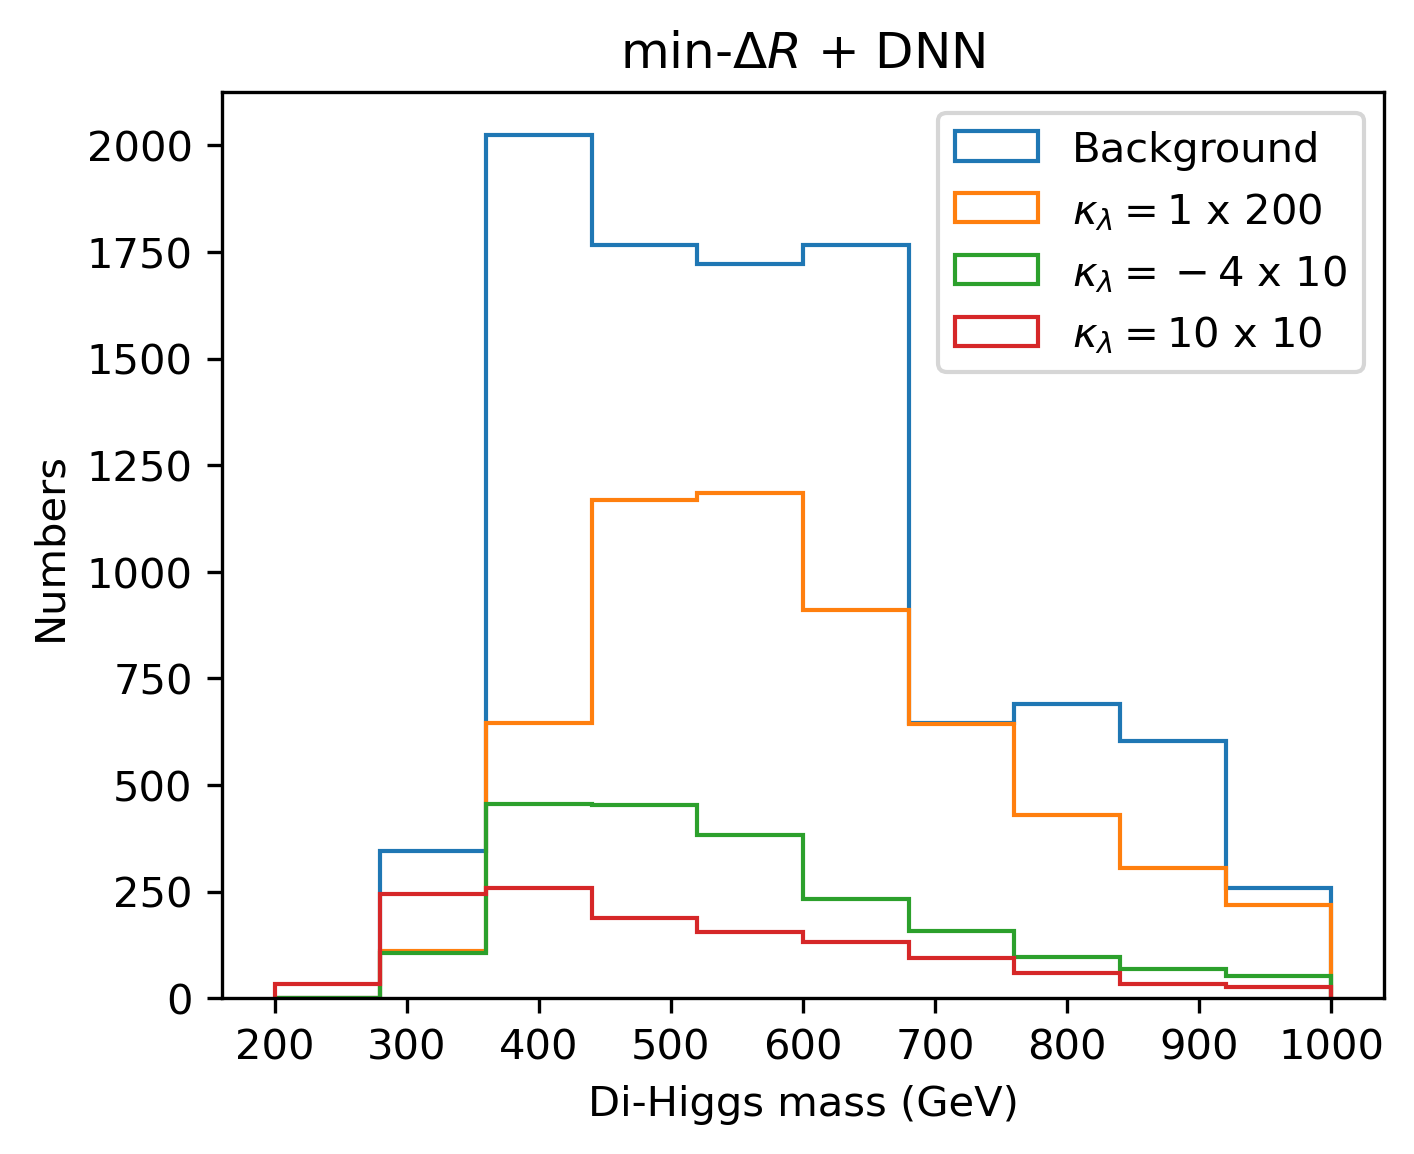
\includegraphics[width=0.30\textwidth]{mhh_DNN_min_dR.png}
			}
			\subfloat[$\kappa 5$ SPANet DNN]{
				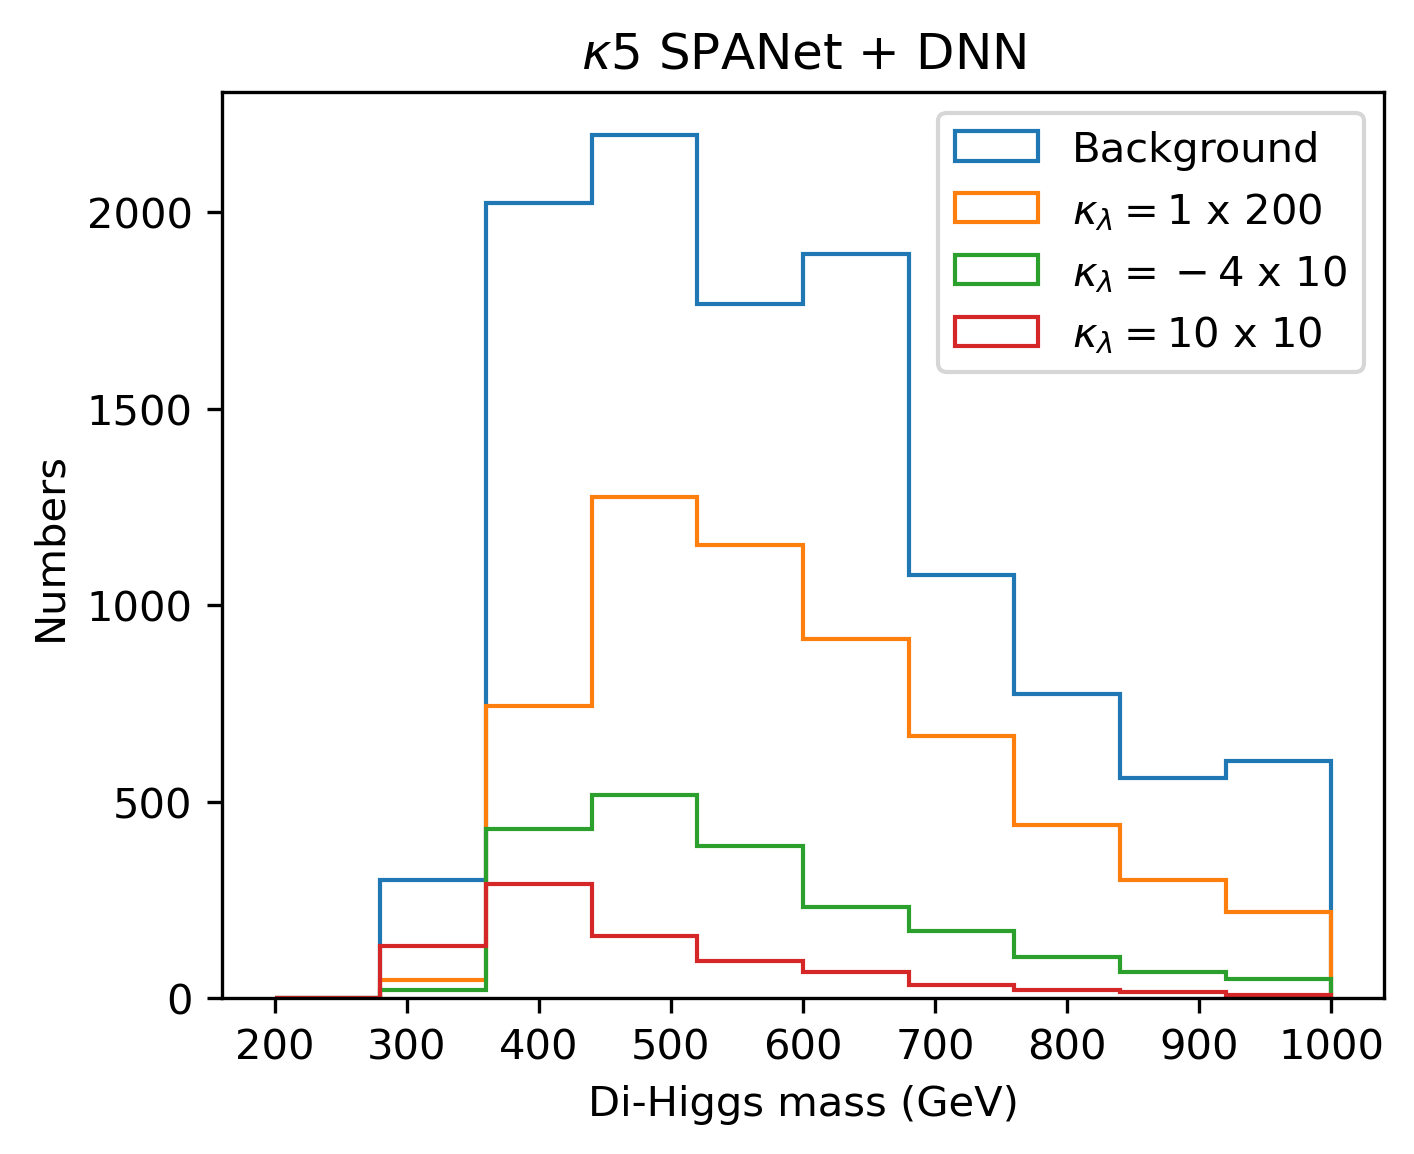
\includegraphics[width=0.30\textwidth]{mhh_DNN_k5_SPANET.png}
			}
			\subfloat[Mixing $\kappa$ SPANet2]{
				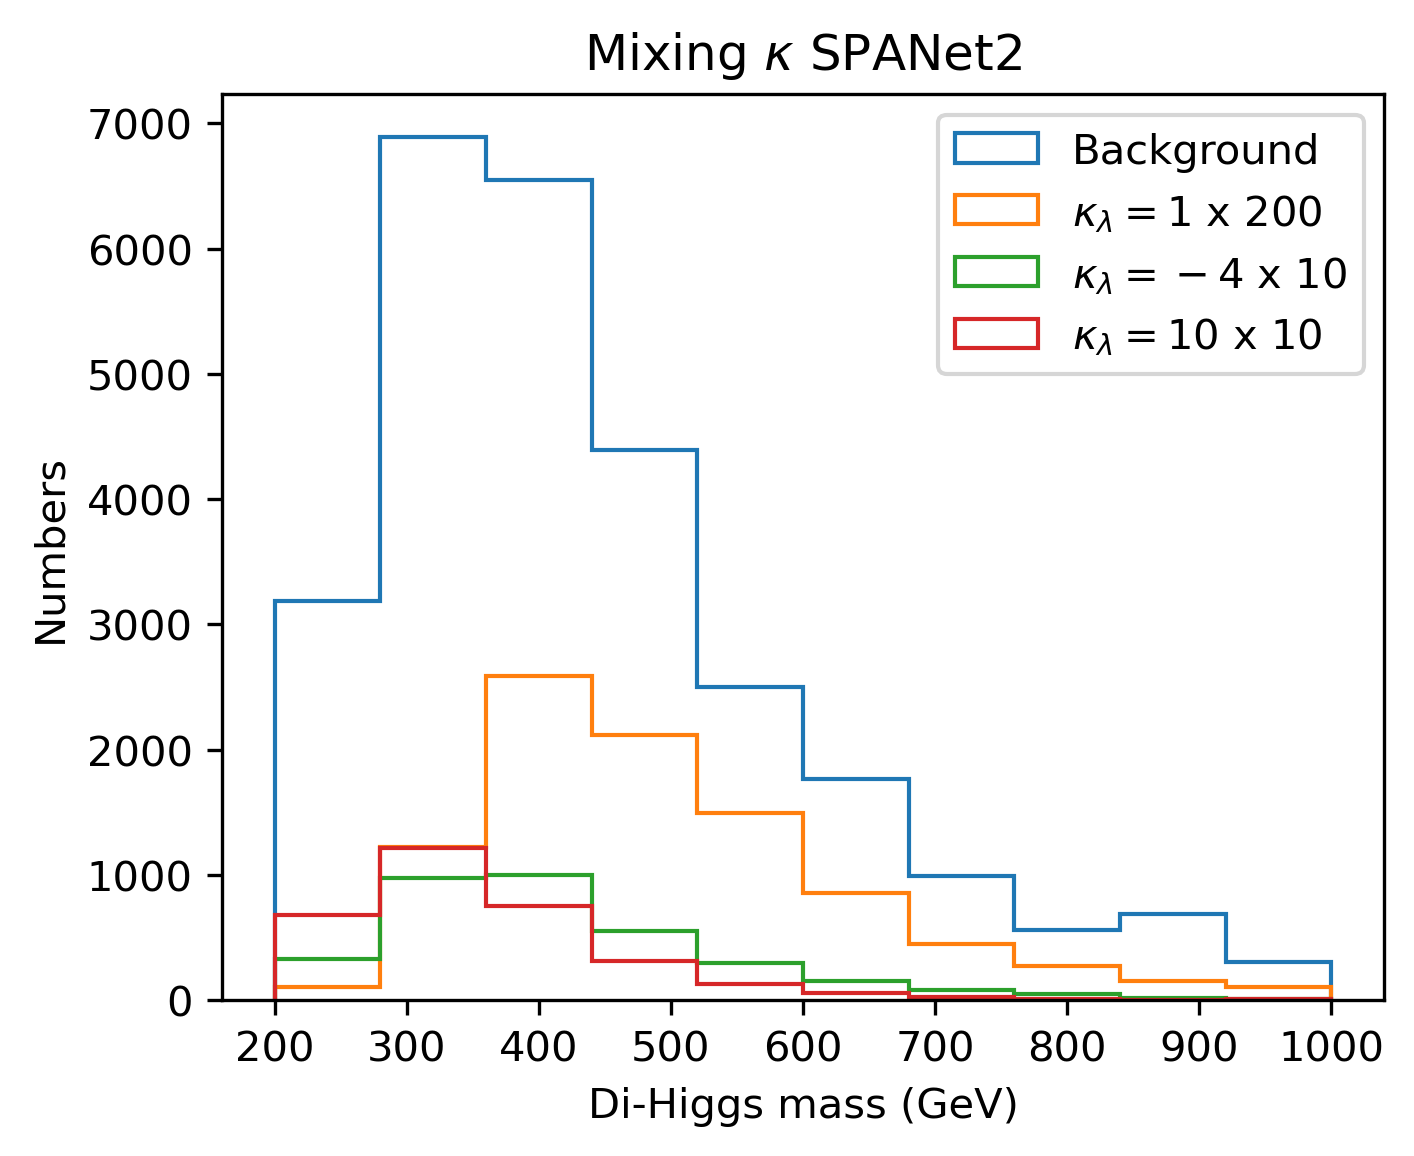
\includegraphics[width=0.30\textwidth]{mhh_mix_SPANET2.png}
			}
			\caption{The $m_{H H}$ distributions after selection. The DNNs are trained with different pairing method samples.}
			\label{fig:mhh_distributions}
		\end{figure}
		
	% subsection mass_distribution_plot (end)
% section comparision_with_previous_results (end)		
\end{document} 

